\documentclass{report}
\usepackage[T1]{fontenc} % Fontes T1
\usepackage[utf8]{inputenc} % Input UTF8
\usepackage[backend=biber, style=ieee]{biblatex} % para usar bibliografia
\usepackage{csquotes}
\usepackage[portuguese]{babel} %Usar língua portuguesa
\usepackage{blindtext} % Gerar texto automaticamente
\usepackage[printonlyused]{acronym}
\usepackage{hyperref} % para autoref
\usepackage{graphicx}
\usepackage{indentfirst}
\bibliography{bibliografia}


\begin{document}
%%
% Definições
%
\def\titulo{Sistemas de Armazenamento de Dados}
\def\data{14/11/2017}
\def\autores{Afonso Cardoso, Pedro Almeida}
\def\autorescontactos{(88964) afonsocardoso@ua.pt, (89205) pedro22@ua.pt}
\def\versao{VERSAO}
\def\departamento{Departamento de Electrónica, Telecomunicações e Informática}
\def\empresa{Universidade De Aveiro}
\def\logotipo{ua.pdf}
%
%%%%%% CAPA %%%%%%
%
\begin{titlepage}

\begin{center}
%
\vspace*{50mm}
%
{\Huge \titulo}\\ 
%
\vspace{10mm}
%
{\Large \empresa}\\
%
\vspace{10mm}
%
{\LARGE \autores}\\ 
%
\vspace{30mm}
%
\begin{figure}[h]
\center
\includegraphics{\logotipo}
\end{figure}
%
\vspace{30mm}
\end{center}
%
\begin{flushright}
\versao
\end{flushright}
\end{titlepage}

%%  Página de Título %%
\title{%
{\Huge\textbf{\titulo}}\\
{\Large \departamento\\ \empresa}
}
%
\author{%
    \autores \\
    \autorescontactos
}
%
\date{\data}
%
\maketitle

\pagenumbering{roman}

%%%%%% RESUMO %%%%%%
\begin{abstract}
Resumo de 200-300 palavras.
\end{abstract}

%%%%%% Agradecimentos %%%%%%
% Segundo glisc deveria aparecer após conclusão...
\renewcommand{\abstractname}{Agradecimentos}
\begin{abstract}
Eventuais agradecimentos.
Comentar bloco caso não existam agradecimentos a fazer.
\end{abstract}

\tableofcontents
% \listoftables     % descomentar se necessário
% \listoffigures    % descomentar se necessário


%%%%%%%%%%%%%%%%%%%%%%%%%%%%%%%
\clearpage
\pagenumbering{arabic}

%%%%%%%%%%%%%%%%%%%%%%%%%%%%%%%%
\chapter{Introdução}
\label{chap.introducao}
%Introduz o tema, apresenta a motivação e finalmente a estrutura.
	Com a evolução da tecnologia e o surgimento das primeiras invenções mecanizadas, surgiu a necessidade de guardar dados e informações importantes. Assim, como resposta a este problema, teve de ser criado algo com a capacidade de registar e guardar essa informação. O que foi criado foram dispositivos de armazenamento de dados, sendo o primeiro o \textit{Punched card} (Cartão perfurado), utilizado pela primeira vez em 1725. 
\vspace{1mm}
	
	Contudo, na atualidade, o armazenamento de dados não é utilizado apenas pelas industrias mas também para utilização pessoal. Todos sentem a necessidade de guardar algo, seja qual for a utilidade ou fim. "Dados são conhecimento, é um pedaço de história, um fragmento de algo ou um todo de uma vida"[1].
\vspace{1mm}
	
	Estes dispositivos de armazenamento têm vindo a sofrer um processo de evolução ininterrupto até aos dias de hoje. Tendo sempre como base as suas origens e como visão, o aumento da sua capacidade de armazenamento, o aumento da velocidade de acesso à informação guardada, assim como, a redução das dimensões físicas dos sistemas de armazenamento.
\vspace{1mm}
	
	Uma alteração que acontece na atualidade em novos computadores, é a substituição do muito usado e comum disco rígido pelo \textit{solid-state drive} (SSD). Assim como este exemplo dado, houve muitas outras inovações que levaram a tecnologia anterior a entrar em desuso, como irá ser descrito com mais pormenor mais à frente.
\vspace{2mm}
%motivaçao	

	Estas evoluções e mudanças na área do armazenamento de dados foi, sem dúvida, o que despertou o interesse para a elaboração deste trabalho, pretendendo, assim, descobrir a origem e a história destes sistemas até aos dias de hoje.
\vspace{2mm}



Este documento está dividido em quatro capítulos.
Depois desta introdução,
no \autoref{chap.metodologia} é apresentada a metodologia seguida,
no \autoref{chap.resultados} são apresentados os resultados obtidos,
sendo estes discutidos no \autoref{chap.analise}.
Finalmente, no \autoref{chap.conclusao} são apresentadas
as conclusões do trabalho.

\chapter{Metodologia}
\label{chap.metodologia}
Descreve os métodos utilizados para obtenção de resultados.

Neste esqueleto de relatório aproveitamos este capítulo para exemplificar
como se usam alguns elementos de {\LaTeX}.

\section{Exemplos}

\subsection{Utilização de acrónimos}
Esta é a primeira invocação do acrónimo \ac{ua}.
E esta é a segunda: \ac{ua}.

Outras duas referências a \ac{miect}
e \ac{miect}.

\subsection{Referências bibliográficas}
Informação relativa à estrutura formal de um relatório pode ser obtida
na página do \ac{glisc}\cite{glisc}.

\newpage
\chapter{Conteúdo}
\label{chap.conteúdo}
	\section{Evolução de Sistemas de Armazenamento de Dados}
		\subsection{Cartão Perfurado}
		O Cartão Perfurado(\textit{Punched Card} foi inventado por Joseph-Marie Jacquard em 1804 para o comando automático de teares depois de ter percebido que as mudanças de linhas coloridas e novelos  seguiam uma certa lógica. Deste modo, Jacquard inventou um processo de cartões perfurados que definiam padrões nas lançadeiras e assim o trabalho do tecelão seria trocado para algo "automático". 
		
		Os cartões perfurados contêm informações digitais representadas pela presença ou falta de furos em posições predefinidas. O método foi interessante para codificar as informações e do ano 1900 a 1950, foram o principal meio de entrada de dados, armazenamento de dados e processamento na computação institucional, tudo pela mão da \textit{International Business Machines} (IBM). 
		
		Apesar de várias melhorias ao longo dos anos, com o desenvolver das tecnologias, os cartões perfurados não conseguiam suprir as necessidades e acabaram por ser substituídos.
		
		\begin{figure}[h]
		\centering
		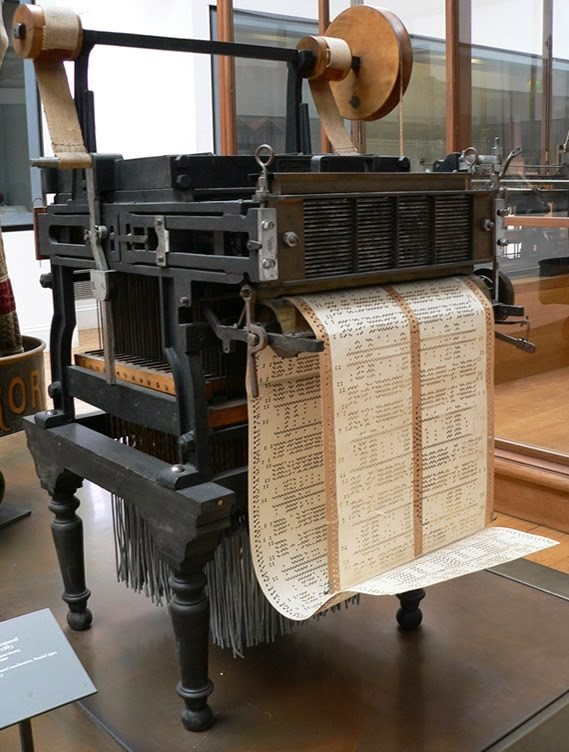
\includegraphics[width=3cm, height=4cm]{cartaoperfurado.jpg}
		\caption{Cartão Perfurado}
		\end{figure}
\newpage

		\subsection{Tubo de Williams}
		O Tubo de Williams é um tipo de memória para computadores criada por Sir Frederick Williams no ano de 1947 na Universidade Manchester tendo sido usado dois anos mais tarde na construção do computador Manchester Mark I.
	
	Este foi o primeiro dispositivo digital de memória de acesso aleatório e foi utilizado com sucesso em vários computadores antigos e possuía uma velocidade de 1,2 milésimos de segundo por instrução, o que na altura era algo bastante inovador.
	
	No seu processo de armazenamento de informação, um eletrão percorre sucessivas linhas na face do tubo, marcando com pontos ou traços de carga elétrica florescente na placa representando assim os uns e os zeros do código binário.
	
	Os primeiros computadores utilizavam este tipo de memória de tubos de raios catódicos (feixes de eletrões), díodo-condensador (mantém a corrente a circular apenas num sentido) e também as memórias de linha de retardo que consistiam num tubo de aproximadamente 150 cm de comprimento contendo mercúrio, com um cristal de quartzo em cada ponta onde os dados a armazenar passavam pelo mercúrio na forma de vibrações mecânicas e eram reconvertidos na outra ponta.
\\

	\begin{figure}[h]
		\centering
		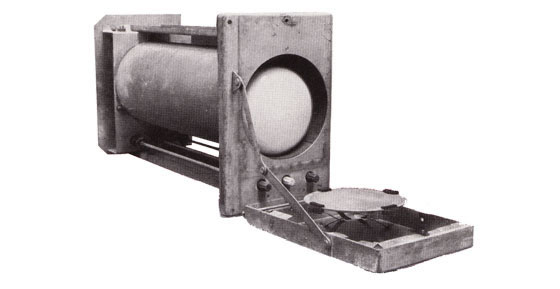
\includegraphics[width=5cm, height=3cm]{williamstube.jpg}
		\caption{Tube de Williams}
		\end{figure}	
\newpage

		
		\subsection{Tambor de Memória}
		 O tambor de memória, também conhecido como\textit{ Drum Memory} foi inventado por Gustav Tauschek em 1932 na Áustria e foi amplamente usado na década de 1950 e na década de 1960.
		 O tambor magnético é constituído por um cilindro de revolução metálico que roda em torno de um eixo vertical e o movimento é assegurado por um motor elétrico. Um conjunto de cabeças fixas assegura a gravação e a leitura da informação
		 
		 A capacidade de armazenamento do tambor de memória original tinha uma capacidade de cerca de 500,000 bits. Este sistema de armazenamento de dados foi especialmente importante pois, no início da década de 60 passaram a utilizar-se na construção de computadores com memórias não voláteis, isto é, não perde a informação guardada depois de desligar a fonte de energia. Estas memórias eram construídas com ferrites e marcam um grande avanço tecnológico na área do armazenamento de dados.
	
	\begin{figure}[h]
		\centering
		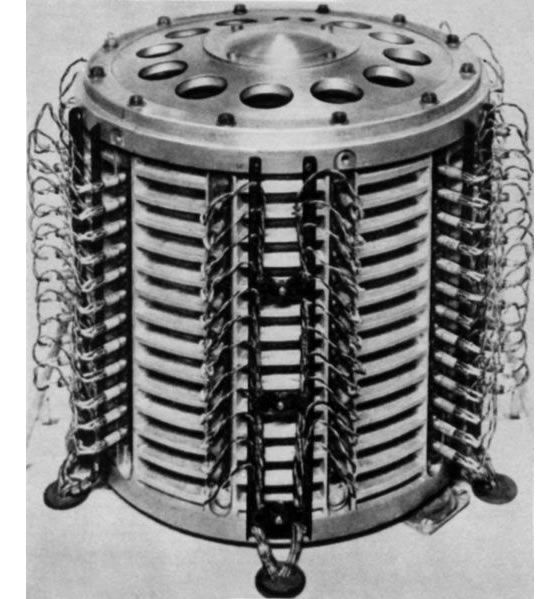
\includegraphics[width=3cm, height=4cm]{tambordememoria.jpg}
		\caption{Tambor de Memória}
		\end{figure}

\newpage
	\subsection{UNISERVO}

	A unidade de fita \textit{UNISERVO}  , introduzido a 1951, foi o principal dispositivo de I/O (os dados entram através de código ou programa para um hardware, assim como a sua saída ou retorno de dados) no computador \textit{UNISERVO I} . O seu lugar ficou garantido na história pois este dispositivo foi a primeira unidade de fita para um computador vendido comercialmente. 
\vspace{1mm}	
	
	O \textit{UNISERVO}  usava uma fita de metal, com 13 mm de largura, feita de uma liga níquel-bronze de fósforo (chamado Vicalloy) e tinha 1200 metros de comprimento, e sendo esta incrivelmente pesada.
\vspace{1mm}
	
	Os dados são guardados em 8 secções da fita, onde 6 são para os valores dos dados (1 ou 0), 1 para a verificação de erros e 1 que regista o tempo, tudo isto à densidade de 128 bits por 2,54 cm. A fita pode ser movida a 254 cm por segundo, oferecendo uma taxa de transferência nominal de 12,800 caracteres por segundo. Os blocos onde os dados são guardados possuem o tamanho fixo de 60 palavras de 12 caracteres cada.
\vspace{1mm}
	
	O \textit{UNISERVO}  ao longo dos anos foi sofrendo várias melhorias e atualizações para ser capaz de ler dados através de outras fitas metálicas.

\begin{figure}[h]
		\centering
		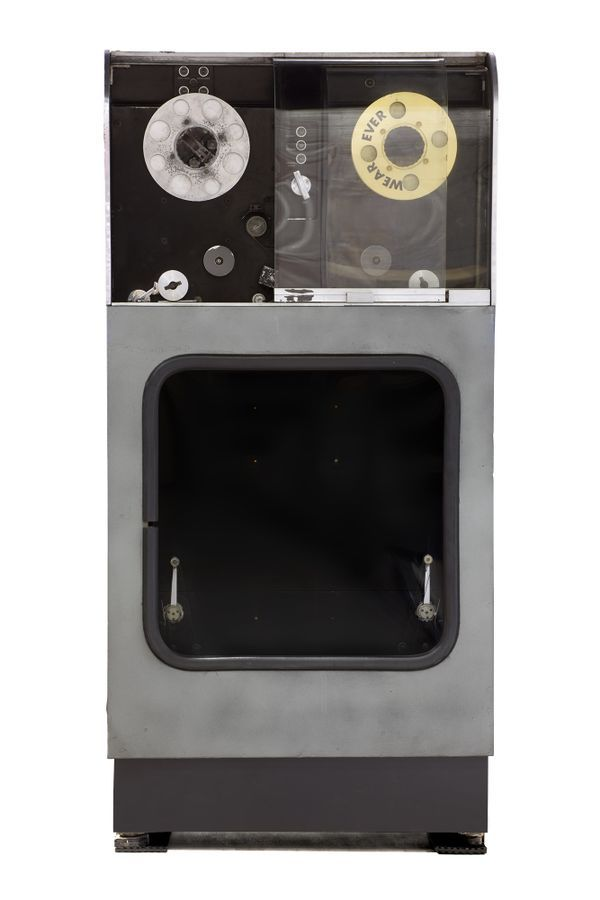
\includegraphics[width=4.7cm, height=7cm]{uniservo.jpg}
		\caption{O UNISERVO}
		\end{figure}
	
\newpage
		\subsection{IBM 350 Disk Storage Unit}
		
		Em 1956, a IBM lançou no mercado o IBM 305 RAMAC(\textit{(Random Access Method of Accounting and Control}), o primeiro computador produzido em série para empresas, visto que até aqui, os computadores eram exclusivos para aplicações militares. Assim, o RAMAC, foi projetado para executar aplicativos de contabilidade e controlo de transações comercias, tais como processamento de pedidos, controlo de inventário e folhas de pagamentos.
\vspace{1mm}

		A novidade que o computador 305 RAMAC, que era equipado com 350 Disk Storage Unit, não era a sua capacidade de processamento, mas na utilização de um novo equipamento periférico para a entrada e saída de dados, o qual permitia a gravação e leitura de dados de forma muito mais rápida comparada com os outros sistemas de armazenamento usados até então.
\vspace{1mm}
		
		A novidade que o computador 305 RAMAC, que era equipado com 350 Disk Storage Unit, não era a sua capacidade de processamento, mas na utilização de um novo equipamento periférico para a entrada e saída de dados, o qual permitia a gravação e leitura de dados de forma muito mais rápida comparada com os outros sistemas de armazenamento usados até então. Ao possibilitar que a informação fosse gravada, lida e alterada em poucos segundos e, principalmente, pudesse ser feito o acesso de forma aleatória, eliminou a necessidade de se classificar os dados em sequência antes do seu processamento, o que até então era um requisito imposto pelos equipamentos de fita magnética ou cartões perfurados, que eram os meios disponíveis para se armazenar dados até ao momento.
\vspace{1mm}

		 O RAMAC pôs fim da era dos cartões perfurados e introduziu uma nova. As corporações passaram a utilizar computadores para realizar negócios, fazendo uso do processamento de transações online e armazenamento de grandes volumes de dados em discos magnéticos. Realçando a importância da tecnologia introduzida no RAMAC e como influenciou por completo no modo de armazenar e processar a informação, ainda na atualidade, apesar de muitos melhoramentos, a tecnologia para produzir discos magnéticos é a mesma. Contudo, 1961 foi o último ano de produção.

	\begin{figure} [h]
		\centering
		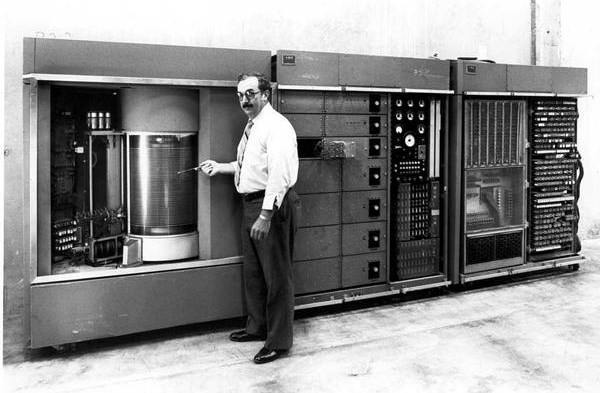
\includegraphics[width=6cm, height=4cm]{RAMAC.jpg}
		\caption{IBM 350 RAMAC}
	\end{figure}
	
\newpage
		
		\subsection{Cassete}	
	A cassete ou \textit{compact cassette}  é um padrão de fita magnética para gravação de áudio lançada oficialmente em 1963, invenção da empresa holandesa \textit{Philips}, possuindo um armazenamento de 660 kB por cada lado da cassete. Possui também a abreviação de: "K7".
\vspace{1mm}
	
	A cassete era constituída basicamente por 2 carretos, a fita magnética e todo o mecanismo de movimento da fita alojados numa caixa plástica. Esta fita é coberta por uma substância à base de ferro, estando presente nesta milhões de ímanes pequenos que formam um campo magnético. Ao gravar dados, as partículas ordenam-se de modo a ser possível a gravação.
\vspace{1mm}

	Isto facilitava o manuseamento e a utilização permitindo que a fita fosse colocada ou retirada em qualquer ponto da reprodução ou gravação sem a necessidade de ser rebobinada como as fitas de rolo. 
\vspace{1mm}
	
	Com um tamanho de 10 por 7 cm, a caixa plástica permitia uma enorme economia de espaço e uma excelente utilização face às fitas tradicionais.
\vspace{1mm}

	No início, era possível gravar apenas 30 minutos em cada lado da fita, perfazendo assim uma hora de gravação. Se usasse mais tempo, a qualidade do som diminuía. Ao longo do tempo, foram acrescentados recursos tecnológicos e as fitas passaram a armazenar conteúdo até 45, 60, 90 e até 120 minutos. A invenção representava uma revolução na época, pois ampliava as possibilidades de reproduzir música, e finalmente, ao surgir os famosos \textit{Walkman}  , fez crescer o aumento de utentes da cassete aumentar drasticamente.
\vspace{1mm}

	Inicialmente a expectativa era de colocar dados neste suporte, mas o seu preço levou a que fosse posta de parte, favorecendo assim o surgimento disquete.
	
	\begin{figure} [h]
		\centering
		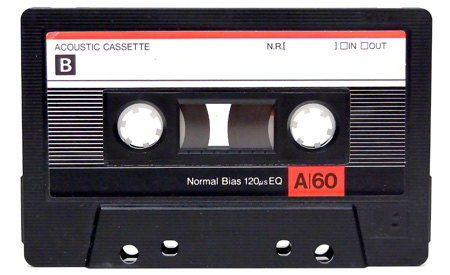
\includegraphics[width=8.19cm, height=5cm]{cassete.jpg}
		\caption{Cassete}
	\end{figure}		
		
\newpage

		\subsection{Disquete}
		A Disquete, também conhecido como \textit{floppy disk}, foi desenvolvida no final da década de 60 mas só ficou disponível comercialmente em 1971 com um tamanho inicial de 8 polegadas e com uma capacidade de armazenamento de dados de 80 kB. Muito resumidamente, uma disquete é um disco protegido por uma capa para evitar que se danifique. 
\vspace{1mm}

		Disquetes podem ser lidas e gravadas por um leitor de disquete, chamado também de \textit{floppy disk drive} (FDD). As disquetes possuem a mesma estrutura de um disco rígido sendo todos periféricos de entrada e saída mas podendo estas ser removíveis e serem compostas apenas por um único disco magnético.
\vspace{1mm}
		
		 Devido à fácil utilização, a disquete foi, por mais de duas décadas, o principal sistema de armazenamento de dados mais utilizado. A maioria dos ambientes computacionais antes de 1990 não possuíam redes, e assim, as disquetes eram o principal sistema de transferência de dados entre os computadores.
\vspace{1mm}
		
		Contudo, vários motivos fizeram com que, com o passar dos anos, as disquetes acabassem em desuso. O principal foi a sua escassa capacidade de armazenamento em comparação com outras tecnologias mais avançadas (embora já tenha sido considerado um dispositivo com grande capacidade de armazenamento) que oferecem como, por exemplo, CD-ROM que irá ser analisado mais tarde. Outra causa para o desuso das disquetes, era a facilidade com que se danificavam fosse por estarem perto de um campo magnético exterior ou por acumulação de sujidade.
\vspace{1mm}
	
		Disquetes podem ser lidas e gravadas por um leitor de disquete, chamado também de \textit{floppy disk drive} (FDD). As disquetes possuem a mesma estrutura de um disco rígido sendo todos periféricos de entrada e saída mas podendo estas ser removíveis e serem compostas apenas por um único disco magnético.
\vspace{1mm}
		
	\begin{table}[h]
		\centering
		\caption{Evolução da Disquete}
		\label{my-label}
		\begin{tabular}{|l|l|l|}
		\hline
		\textbf{Tipo de Disco} & \textbf{Ano} & \textbf{Capacidade} \\ \hline
		8 pol            & 1971 & 80 kB   \\ \hline
		8 pol            & 1973 & 256 kB  \\ \hline
		8 pol            & 1974 & 800 kB  \\ \hline
		8 pol dual-sided & 1975 & 1 MB    \\ \hline
		1.25 pol         & 1976 & 160 kB  \\ \hline
		1.25 pol         & 1978 & 360 kB  \\ \hline
		1.25 pol         & 1980 & 720 kB  \\ \hline
		1.25 pol         & 1984 & 1.2 MB  \\ \hline
		3 pol            & 1984 & 320 kB  \\ \hline
		1.5 pol          & 1984 & 720 kB  \\ \hline
		1.5 pol          & 1987 & 1.44 MB \\ \hline
		1.5 pol          & 1991 & 2.88 MB \\ \hline
		1.5 pol          & 1993 & 5.76 MB \\ \hline
		
		\end{tabular}
		\end{table}		
 
	Analisando a tabela, pode concluir-se que, ao longo dos anos, a dimensão física tem tendência a diminuir, inversamente à capacidade de armazenamento de dados que vai aumentando. A disquete passou também a ler dados em vez de só os gravar. 

	\textbf{Fato:}	
		\begin{itemize}
		 	\item Os disquetes foram os primeiros transmissores de vírus de computador. 
	 	\end{itemize}
	
	
	\begin{figure} [h]
		\centering
		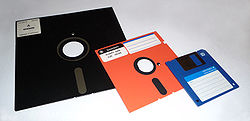
\includegraphics[scale=1]{disquete.jpg}
		\caption{Disquete}
	\end{figure}
	
\newpage		
		
		\subsection{IBM 3380}
	
	O IBM 3380 \textit{Direct Access Storage Device}  foi introduzido em Junho de 1980. Usa uma nova cabeça de leitura e tinha uma capacidade de 2.52 GB, com uma taxa de 3 MB por segundo de transferência de dados. O tempo médio de acesso era de 16 ms (milissegundos). Preço de compra no momento da introdução variou de 81,000 dólares a 142,200 dólares.
\vspace{1mm}

	Este foi o primeiro dispositivo de armazenamento a atingir o reino do Gigabyte. Fica assim na história por esse feito.
\vspace{1mm}

=======
		\subsection{IBM 3380}	
	O IBM 3380 \textit{Direct Access Storage Device}  foi anunciado em Junho de 1980 pela IBM. Foi desenvolvido pela Universidade de Auckland e foi o primeiro dispositivo de armazenamento a atingir o território do Gigabyte, ficando ,assim, na história por esse mesmo feito.
	
	Os vários modelos da série 3380 ((A4, A4F, AA4, AAF, B4 e BF4), eram uma apenas uma solução de armazenamento de dados, não eram o próprio computador. Todos esses modelos usavam duas \textit{hard drives} com cerca de 1.26 GB cada, perfazendo, assim, um total de 2.52 GB. Tinha uma taxa de 3 MB por segundo de transferência de dados. O tempo médio de acesso era de 16 ms (milissegundos). O seu peso era de aproximadamente 29 kg. 
	
	Apesar dos vários modelos da série 3380 terem todas características semelhantes, foram sempre recebendo melhoramentos. Comparando o primeiro modelo com o último, foi possível reduzir o consumo de energia em 70\% e a produção de calor em 75\%. Estes avanços, fizeram com que o IBM 3380 se tornasse muito mais fiável e eficiente.
	
	O preço de adquirição deste equipamento no momento em que foi introduzido no mercado variou de 81,000 dólares a 142,200 dólares, dependendo do modelo.
\vspace{1mm}

	\begin{figure} [h]
		\centering
		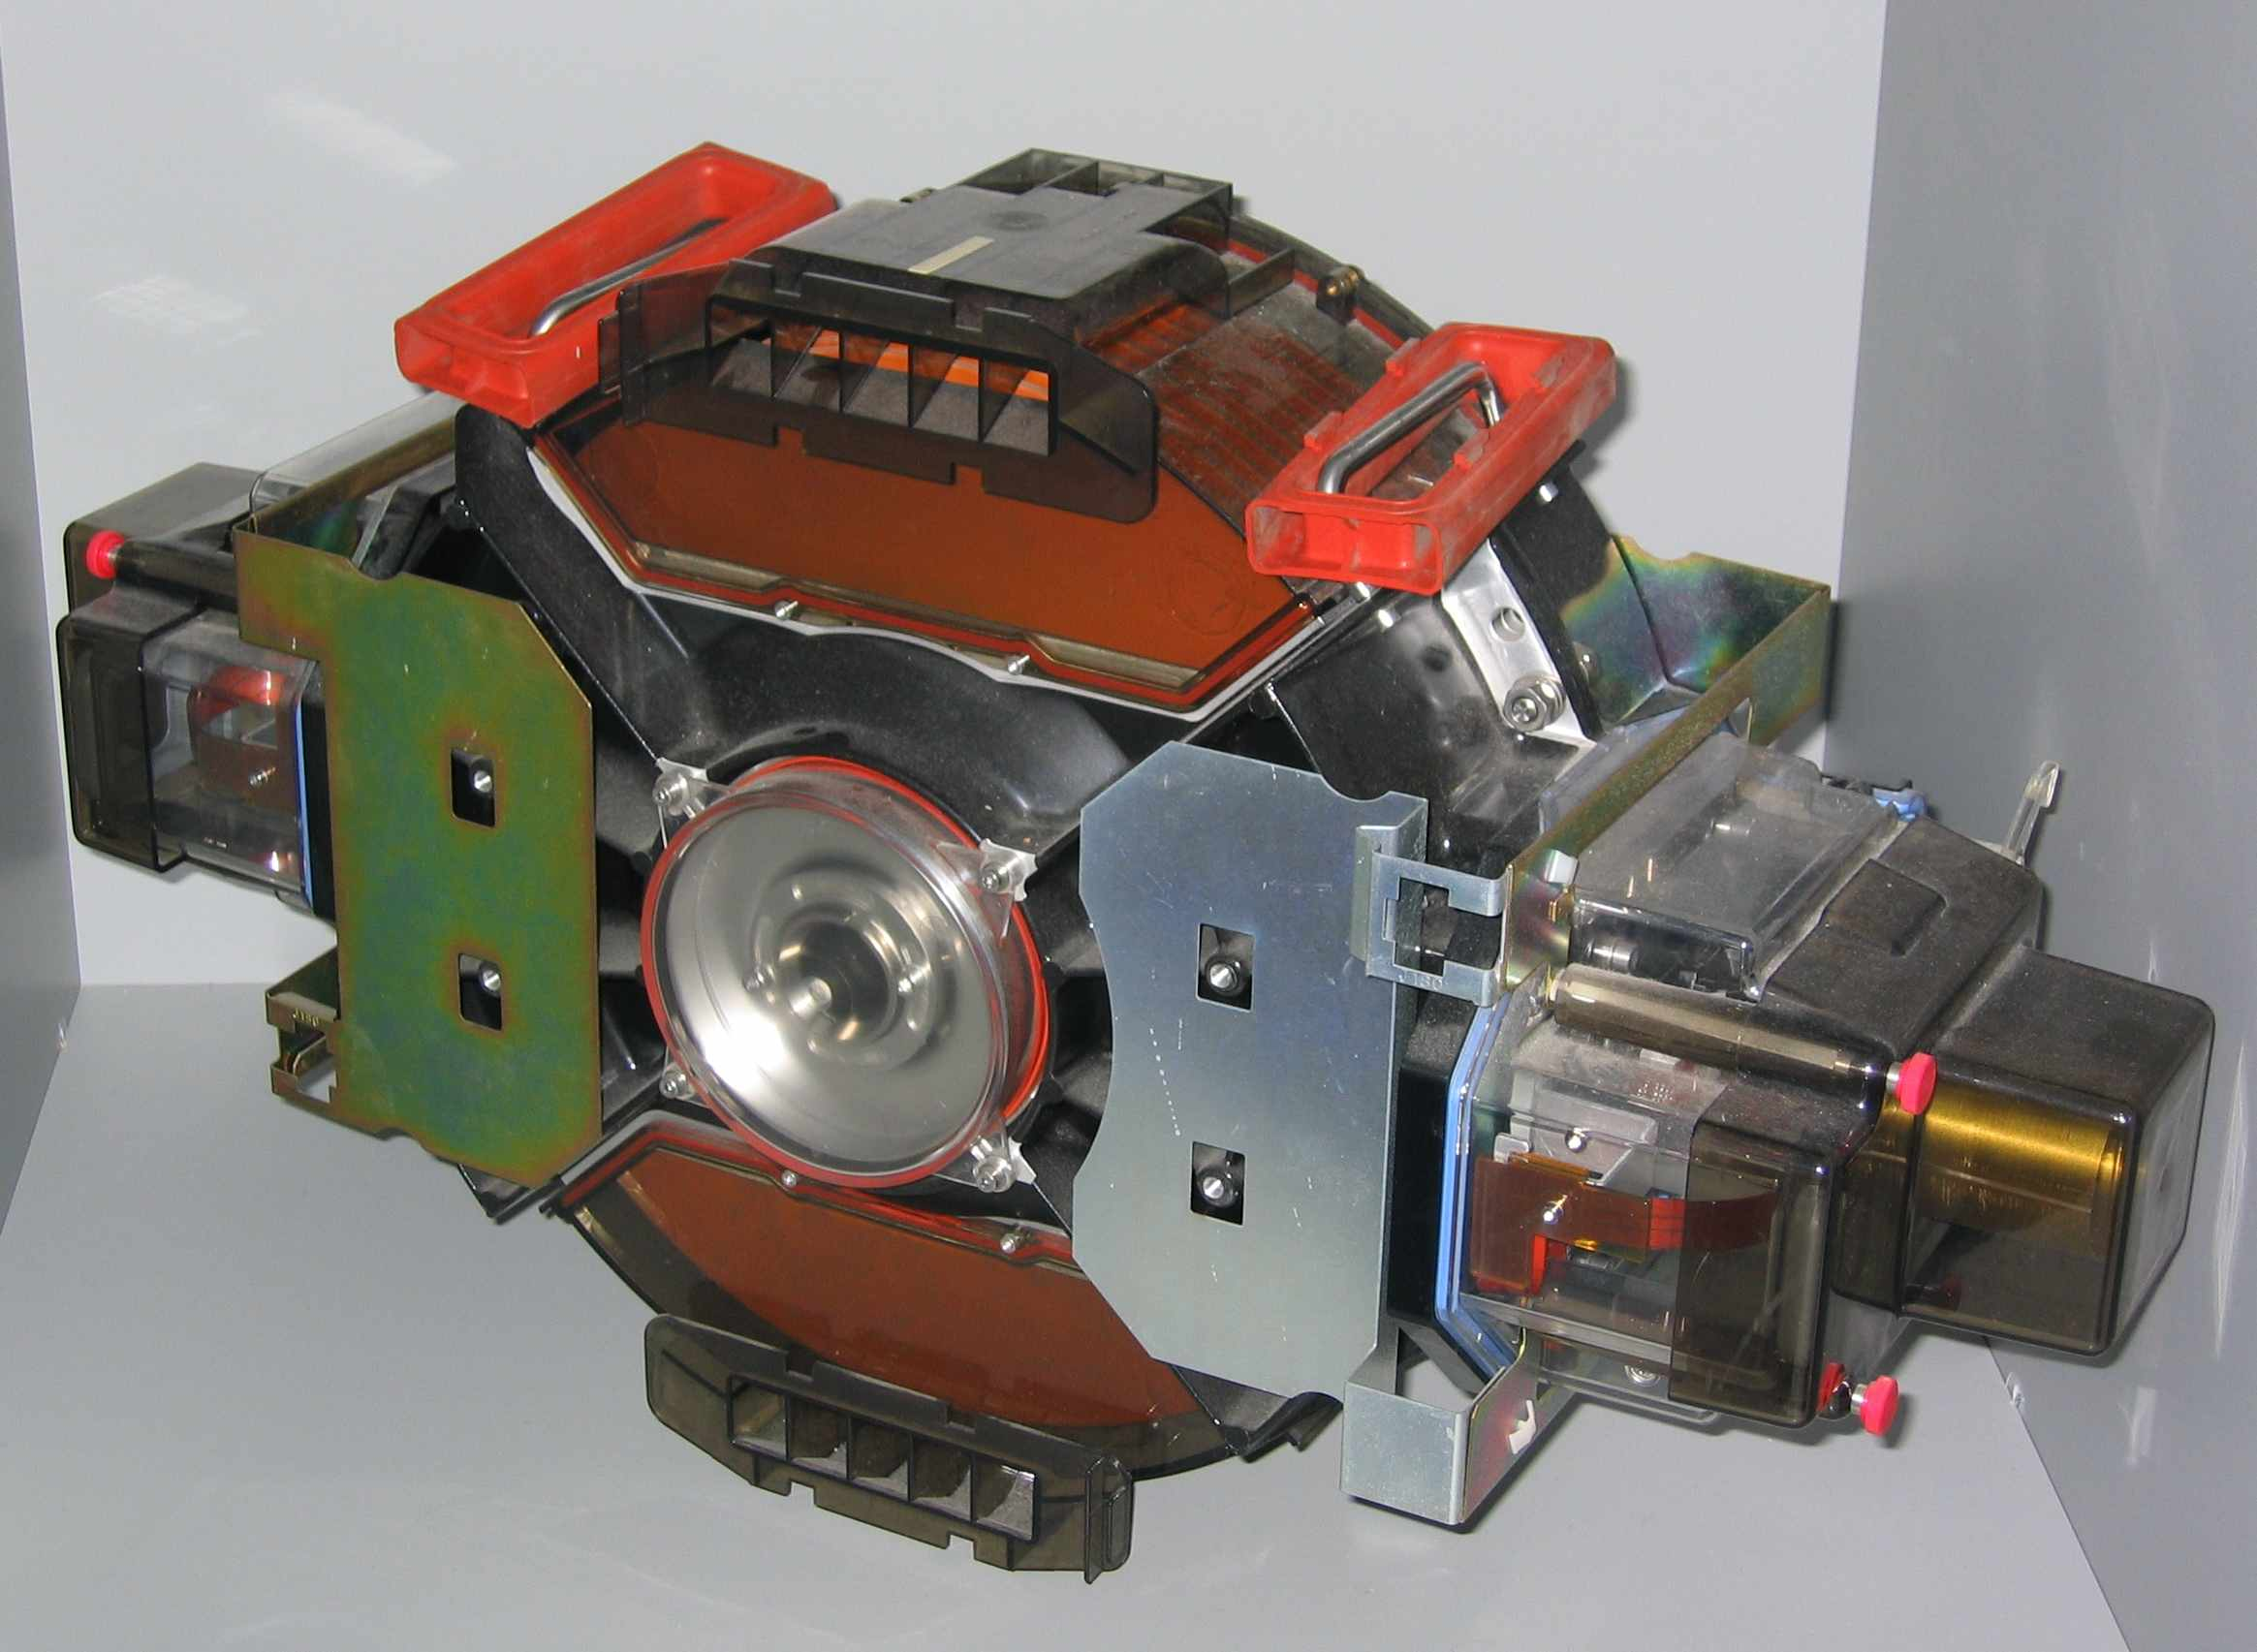
\includegraphics[scale=0.07]{ibm3380.jpg}
		\caption{Hard Drive Assembly (HDA)}
	\end{figure}

\newpage
		
		\subsection{ST-506}

	O ST-506 foi o primeiro disco rígido de 5.25 polegadas. Apresentado em 1980 pela então denominada \textit{Shugart Technology} (hoje \textit{Seagate Technology}), tinha uma capacidade de 5 MB após formatação. 
\vspace{1mm}

	O ST-412 um modelo semelhante, mas muito mais caro, tinha um espaço de armazenamento de 10 MB e foi lançado em fins de 1981. Ambos usavam codificação MFM (um esquema de coficação em linha para codifcar informação na maioria dos modelos da disquete unidades de disquete).
\vspace{1mm}
	
	Uma versão posterior do ST-412 usava RLL (uma técnica de codificação em linha que foi usada para enviar dados arbitrários por um canal de comunicações com largura de banda limitada) para um incremento de 50\% na capacidade e taxa de transferência.
\vspace{1mm}
	
	Esta foi a primeira drive com esta dimensão e foi quem deu origem aos atuais discos rígidos que hoje conhecemos e usamos tão frequentemente.
\vspace{1mm}

	O ST-506 estava presente na interface de um computador usando um controlador de disco. A interface do ST-506 era derivada da interface SA1000 da \textit{Shugart Associates}  a qual por sua vez era baseada na interface da unidade de disquetes tornando assim a fabricação de controladores de disco relativamente fácil.
\vspace{1mm}

	\begin{figure} [h]
		\centering
		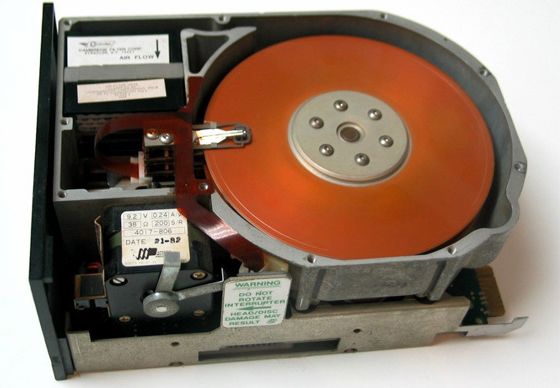
\includegraphics[scale=0.3]{st-506.jpg}
		\caption{O ST-506}
	\end{figure}		
		
%\chapter{Análise}
%\label{chap.analise}
%Analisa os resultados.

\chapter{Conclusões}
\label{chap.conclusao}
Apresenta conclusões.

\chapter*{Contribuições dos autores}
Resumir aqui o que cada autor fez no trabalho.
Usar abreviaturas para identificar os autores,
por exemplo AS para António Silva.
No fim indicar a percentagem de contribuição de cada autor.

%%%%%%%%%%%%%%%%%%%%%%%%%%%%%%%%%
\chapter*{Acrónimos}
\begin{acronym}
\acro{ua}[UA]{Universidade de Aveiro}
\acro{miect}[MIECT]{Mestrado Integrado em Engenharia de Computadores e Telemática}
\acro{lei}[LEI]{Licenciatura em Engenharia Informática}
\acro{glisc}[GLISC]{Grey Literature International Steering Committee}
\end{acronym}


%%%%%%%%%%%%%%%%%%%%%%%%%%%%%%%%%
\printbibliography

\end{document}
